\section{Methodology} \label{sec:methodology}

Throughout this section, the selected architectures for the blind super resolution task will be explained in-depth, along with the rationale behind their choice. Additionally, all the metrics and losses used during training and experimentation will be introduced. 
Moreover, a process to create a baseline dataset to assess the performance of the selected architecture is explained in detail. 


\subsection{Models architecture}

\subsubsection{Probabilistic degradation model}

    The probabilistic degradation model architecture, introduced in \cite{luo2022learning}, is classified among implicit modeling methods for blind super resolution.
    Typically, models in this category aim to learn the degradation process adaptively through deterministic models. Nevertheless, specific degradations in practical scenarios show stochastic behavior and do not strictly correlate with the image's content. Such methods may struggle to capture these unpredictable elements and the content-independent aspects of degradation, potentially constraining the performance of the subsequent SR model. In this particular architecture, the degradation \(D\) is assumed as a random variable, and two networks seek to learn its distribution by mapping two random variables $z_k$ and $z_n$ to \(D\). 

    Contrary to previous models that use deep learning to directly transform an HR image into an LR one, this strategy employs two networks to generate a blurring kernel and additive noise, following Eq. \ref{eq:2-degradation-equation}. This constraint imposes limitations on how the degradation affects the images, thus making its integration with an SR model easier and allowing efficient end-to-end training. Additionally, it provides actionable insight into understanding the unknown degradation process.
    The stochastic nature of the model allows the production of a wider variety of degradations, thereby allowing the creation of diverse HR-LR pairs. This diversity covers the possible degradations in test LR images and prevents the SR model from overfitting to specific scenarios.

    
    The degradation is parametrized using two random variables, the blur kernel $k$ and random noise $n$, by formulating the degradation process as the linear function from Eq. \ref{eq:2-degradation-equation}.
    The equation can be divided into two linear steps \cite{zhu2020unpaired}: 

    \begin{equation}
        \begin{aligned}
                I^{\text{LR}}_{\text{clean}} &= (I^{\text{HR}} * k) \downarrow_s \\
                I^{\text{LR}} &= I^{\text{LR}}_{\text{clean}} + n
        \end{aligned}
    \end{equation}
    
    In most cases, the two steps are mutually independent, as the blur kernels are mainly dependent on the properties of the camera lens, and the noises are primarily related to the properties of sensors. 
    Thus, the distribution of the degradation process can be represented as the product of the distribution of $k$ and $n$, which can be modeled by learning the mapping from random variable $z_k$ and $z_n$ to $k$ and $n$, respectively.


    \begin{equation}
        p_{D}(D) = p_{k,n}(k, n) = p_{k}(k)p_{n}(n).
    \end{equation}

    To model the distribution of the blur kernel k, a random variable $z_k$, which is subject to a multi-dimensional normal distribution, is defined. 
    Then, a generative module is used to learn the mapping from $z_k$ to $k$. 

    \begin{equation}
        k = \text{net}K(z_k), \quad z_k \sim \mathcal{N}(0,1),
    \end{equation}

    The spatially variant blur kernel is considered first. This implies that the blur kernel for each pixel of the image is different. In that case, the shapes of $z_k$ and $k$ are:

    \begin{equation}
        z_k \in \mathbb{R}^{f_k \times H \times W}, \quad k \in \mathbb{R}^{(k \times k) \times H \times W},
    \end{equation}

    Where $f_k$ is the dimension of the normal distribution $z_k$ and $k$ is the size of the blur kernel. $H$ and $W$ represent the height and width of the image, respectively.
    Generally, the sizes of the convolutional weights are set as 3 × 3, which indicates that the learned blur kernels of neighboring pixels are spatially correlated.
    If the spatial size of all convolutional weights is set as 1 × 1, the blur kernel could be approximated by a spatially invariant one, which is a particular case of the spatially variant blur kernel with $H = W = 1$.
    This approximation simplifies the dimensions of the problem drastically and is an appropriate assumption if the crops used for training the model are small.
    A softmax layer is added at the end of the network to guarantee that the sum of all elements of $k$ equals to one.
    
    
    To model the distribution of the noise $n$, a  generative module can also be used:

    \begin{equation}
        n = \text{net}N(z_n), \quad z_n \sim \mathcal{N}(0,1),
    \end{equation}

    \begin{equation}
        z_n \in \mathbb{R}^{f_n \times H \times W}, \quad n \in \mathbb{R}^{C \times H \times W },
    \end{equation}

    Where the height, width, and number of channels of the image are noted as $H$, $W$, and $C$, respectively. 
    In this work, $C$ is always set to 1.

    In other methods \cite{plotz2017benchmarking}, the noise is modeled as a combination of shot and read noise. 
    It can be approximated as a heteroscedastic Gaussian distribution, which is dependent on the content of the image:

    \begin{equation}
        n \sim \mathcal{N}(0, \sigma_{\text{read}} + \sigma_{\text{shot}} \cdot I^{\text{LR}}_{\text{clean}}),
    \end{equation}

    This indicates that the noise is also related to the image content, and the distribution of $n$ should be expressed as:


    \begin{equation}
        n = \text{net}N(z_n,I^{\text{LR}}_{\text{clean}}), \quad z_n \sim \mathcal{N}(0,1),
    \end{equation}

    \begin{figure}[h!]
        \centering
        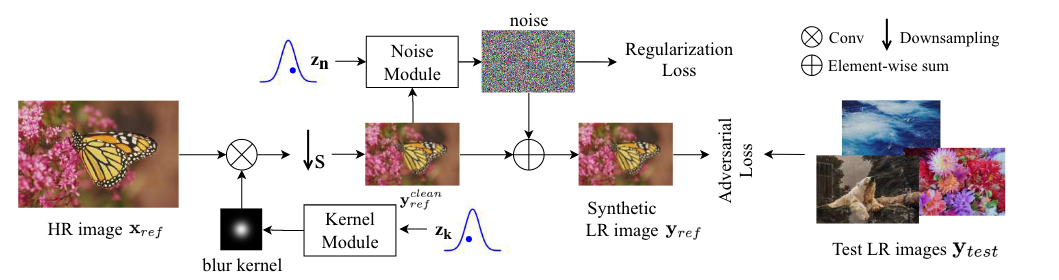
\includegraphics[width=\textwidth]{Includes/3-probabilistic-degradation-model.png}
        \caption{Schematic of the probabilistic degradation module.
                The discriminator is left out for a more intuitive description (source: \cite{luo2022learning}).}
        \label{fig:3-probabilistic-degradation-model}
    \end{figure}

    The probabilistic degradation model is optimized via adversarial training, which encourages the output of the generator to be similar to the test LR images \cite{bulat2018learn}.
    To avoid overly noisy images, a constraint to the noise level is added to the loss function via a regularization term. 
    A multiplication constant is also added to balance the magnitude of the two terms.

    \begin{equation}
        \mathcal{L}_{\text{total}} = \mathcal{L}_{\text{adversarial}} + 100 \cdot \|n\|_2^2.
    \end{equation}

    This approach formulates the degradation process as a linear function, and the learned degradations can only impose a limited influence on the image content.
    This way, it decouples the degradations with image content better and it places the focus on learning the degradations.
    This limitation imposed on the generator eliminates the need for guidance using a bicubically downscaled version of the HR image, as opposed to \cite{wei2020unsupervised} or \cite{bulat2018learn}.

    \begin{figure}[H]
        \centering
        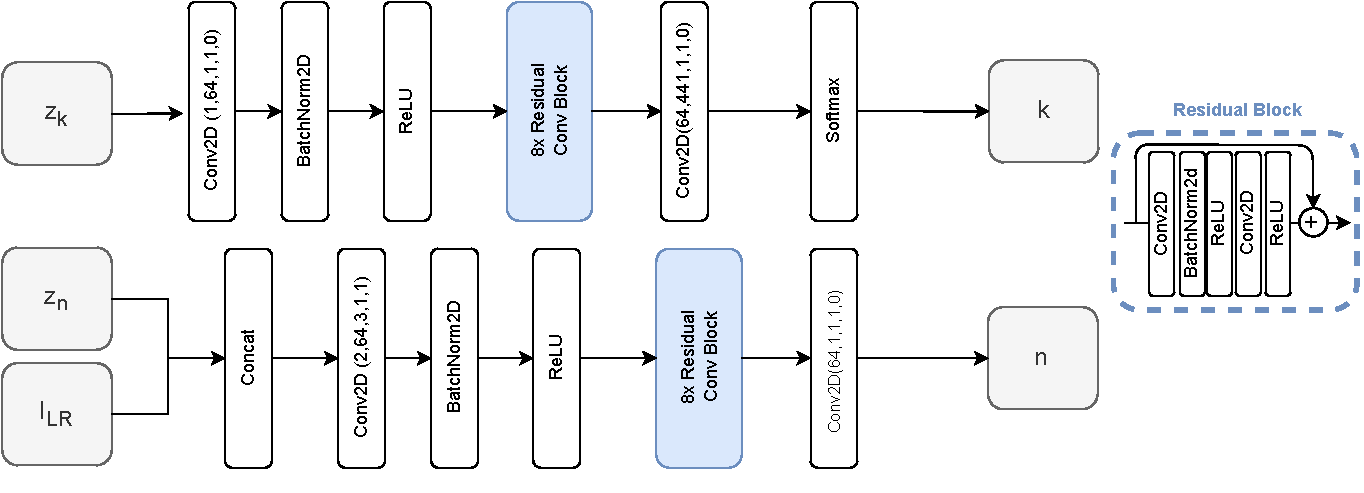
\includegraphics[width=\textwidth]{Includes/3-slim-gen-module.pdf}
        \caption{Schematic of the generative networks used in the kernel and noise module of the probabilistic degradation model.
        The parameters of the convolutional layers represent input channels, output channels, kernel size, stride, and padding, respectively.
        The residual blocks use the same kernel size as the convolutional layers of each module.}
        \label{fig:3-slim-gen-module}
    \end{figure}

    To discriminate the generated images from the test images, a PatchGAN discriminator is used \cite{isola2018imagetoimage}. This architecture assesses the structure of local image patches, allowing it to focus on high-frequency details of the image. This is particularly useful in the context of this approach, where the generated images are expected to share a lot of information in the low frequencies of the domain, and the differences with the real LR images are expected to be in the high frequencies. The architecture of the discriminator is shown in Fig. \ref{fig:3-slim-patchgan-module}.
    The network seeks to classify patches of an image as real or fake. The size of the patches depends mainly on the number of strided convolutional layers that are employed. The discriminator outputs a matrix of values, where each value represents the probability that the corresponding patch is real. The final output is obtained by averaging the values in the matrix.

    \begin{figure}[H]
        \centering
        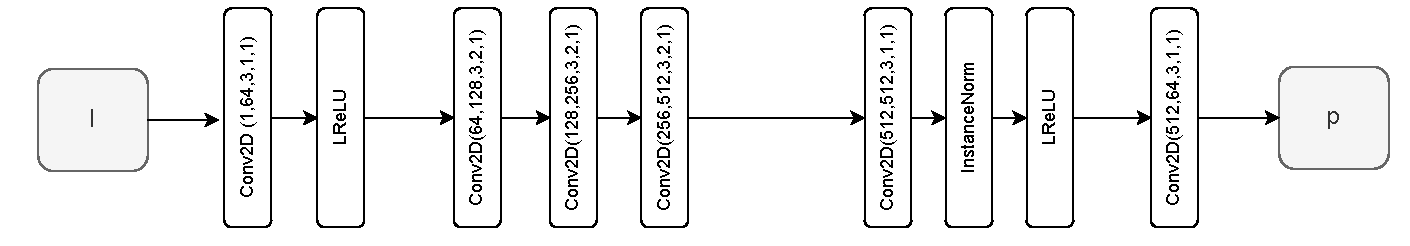
\includegraphics[width=\textwidth]{Includes/3-slim_patchGAN_architecture.pdf}
        \caption{Diagram of the PatchGAN discriminator.
                 The parameters of the convolutional layers represent input channels, output channels, kernel size, stride, and padding, respectively. }
        \label{fig:3-slim-patchgan-module}
    \end{figure}

    
    The constrained nature of the probabilistic degradation model allows the possibility to train it simultaneously with a super resolution algorithm, as described in Fig. \ref{fig:3-GAN-degradation-model}.      
    This way, it can be integrated with any SR model to form a unified framework for blind SR that can be trained in an end-to-end fashion, allowing faster iterations.
    Other methods \cite{fritsche2019frequency,wei2020unsupervised} require that the training of the degradation model and the SR model be in separate phases. First they train a degradation model and then use the trained degradation model to generate pairs and train the SR model.
    This two-step training method is time-consuming but necessary because the highly nonlinear degradation models used will produce undesirable results at the beginning of the training, which may mislead the optimization of the SR model.

    \begin{figure}[H]
        \centering
        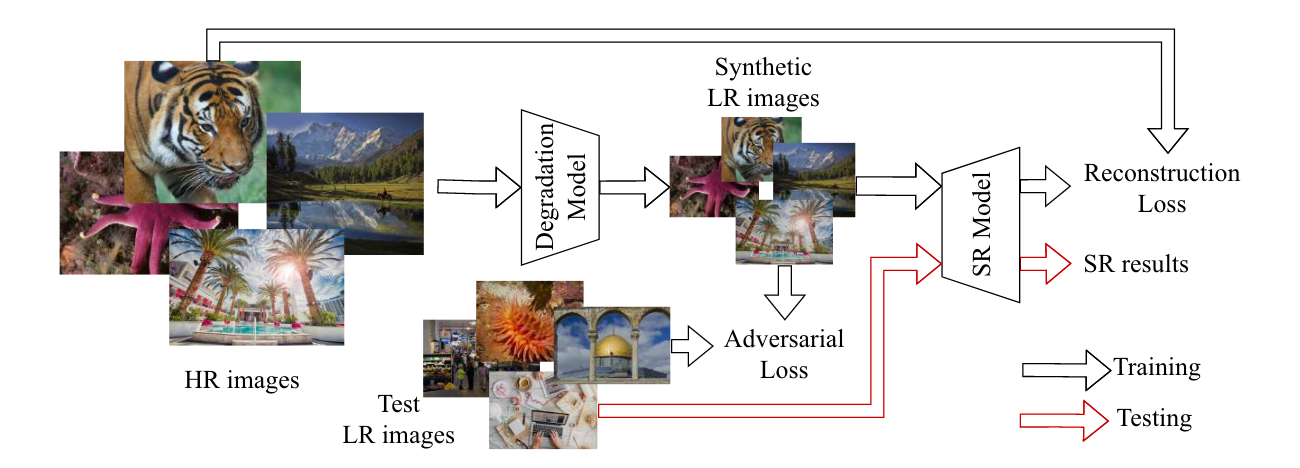
\includegraphics[width=\textwidth]{Includes/3-GAN-degradation-model.png}
        \caption{The probabilistic degradation model is used to encourage the degradation model to produce images in the same domain as the test LR images.
                After training, the SR model is directly used to process the inputs (source \cite{luo2022learning}).}
        \label{fig:3-GAN-degradation-model}
    \end{figure}

    The probabilistic degradation model constitutes a flexible framework for blind super resolution. 
    The only data requirement is a big enough unpaired dataset of LR and HR images and an optional smaller paired dataset for validation and early stopping of the model training.
    The most significant limitation of this approach is the one that implicit modeling methods have: the HR images (source domain) and the LR images (target domain) must be well defined for the model to generalize to a domain that is not in the datasets. 
    Using this framework for general images is difficult due to the variety of cameras, sensors, and compression algorithms that play a part in image distribution. Nevertheless, in the context of this study, the remote sensing images are characterized by a well-defined degradation process that remains relatively stable over time.


\subsubsection{SRResNet}

    
    The SRResNet architecture is used to perform the super resolution task. This network has been used extensively in the literature and has proven to be a good baseline for SR. It can also be easily extended for multi-spectral super resolution, as in \cite{myself2023}. It uses a residual network architecture in a post-upsampling framework based on sub-pixel convolution layers.
    
    Introduced in 2017 \cite{ledig2017photorealistic}, SRResnet is the generator in the SRGAN architecture, which is a GAN-based super resolution method. The purpose of the GAN is to drive the reconstruction process towards the natural image manifold, producing more visually convincing solutions. Additionally, a perceptual loss based on activation layers of a pre-trained VGG network \cite{simonyan2015deep} is incorporated into the pixel loss training objective. As this work focuses on having super-resolved images with high physical consistency and not on the perceptual superiority of the images, these two components are left out,  keeping only the generator and the pixel loss. The architecture, with slight modifications, is detailed in Fig. \ref{fig:3-resnet-architecture}.

    First, features are extracted from the input using a convolutional layer with 64 filters and a kernel size of 3, plus a ParametricReLU activation function.
    Before going through the core of the network, the feature map is reduced by half using a 1x1 convolutional layer.
    The core of the network is composed of five residual blocks, consisting of two convolutional layers, followed by batch-normalization layers and ParametricReLU activation functions. 
    The convolutional layers have 3x3 kernels and sixty-four feature maps. 
    Two trained sub-pixel convolution layers are used to increase the resolution of the input image.

    \begin{figure}[H]
        \centering
        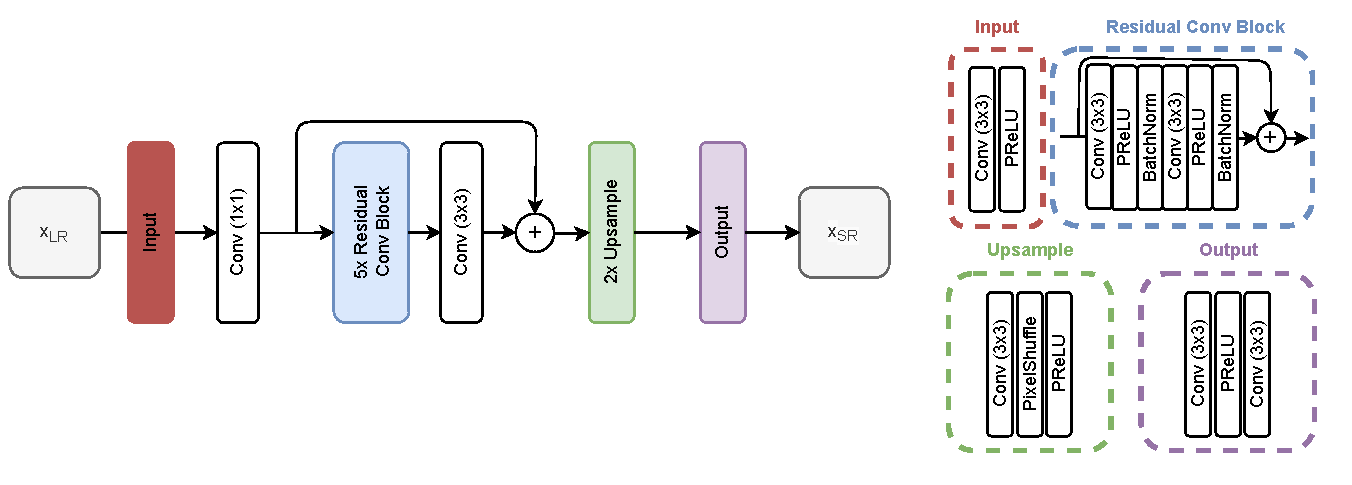
\includegraphics[width=1\textwidth]{Includes/3-srresnet-architecture.pdf}
        \caption{ Modified SRResNet architecture. $X_{LR}$ represents the LR input image, $X_{SR}$ the super-resolved image, which is then compared to the ground truth $X_{HR}$.}
        \label{fig:3-resnet-architecture}
     \end{figure}
    
    \subsection{Baseline degradation model} \label{subsec:baseline_degradation_model}

        As stated in \ref{subsec:domaingap}, early super-resolution methods commonly generated paired HR-LR samples using predefined degradation techniques, with bicubic downsampling being the most used setting \cite{zhang2018residual}.
        This kind of synthetic data, while easy to obtain, often results in a domain gap problem, where the data used for training and assessing the model do not come from the same distribution as the real data. This gap usually leads to decreased performance when the models are deployed in production environments.
        
        A possible solution is to synthesize samples with a stochastic degradation model, which includes a set of multiple blurring kernels and several random noise configurations that convert scenes from an HR mission into LR versions.
        The larger degradation space grants these models better generalization capabilities and lets experts be part of the kernel definition process based on prior knowledge of the degradation process.
        However, the variety of predefined degradations is limited and still fails in most applications. A degradation model like this one will be used to generate a baseline dataset for this work.
        

        \subsubsection{Blurring kernel}

        In the literature, the kernel of the degradation process is usually modeled as a fixed isotropic Gaussian kernel, with a parameter $\sigma$ that depends on the scale factor of the super resolution process.
        To provide more variability to each dataset pair, the parameters of the blurring kernel that determine its width in both axes, $\sigma_x$ and $\sigma_y$, are sampled from a normal distribution with a determined mean and standard deviation. Fig. \ref{fig:4-degradation_kernels} shows some examples of kernels generated using this method; in the upper row, both distributions have a similar mean and variance, resulting in approximate isotropic kernels. In the lower row, the mean of the x-axis is much higher than the mean of the y-axis, resulting in anisotropic kernels. The effects of these kernels on the HR-LR generation are shown in Fig. \ref{fig:4-degradation-kernel-examples}.



        \begin{figure}[H]
                \centering
                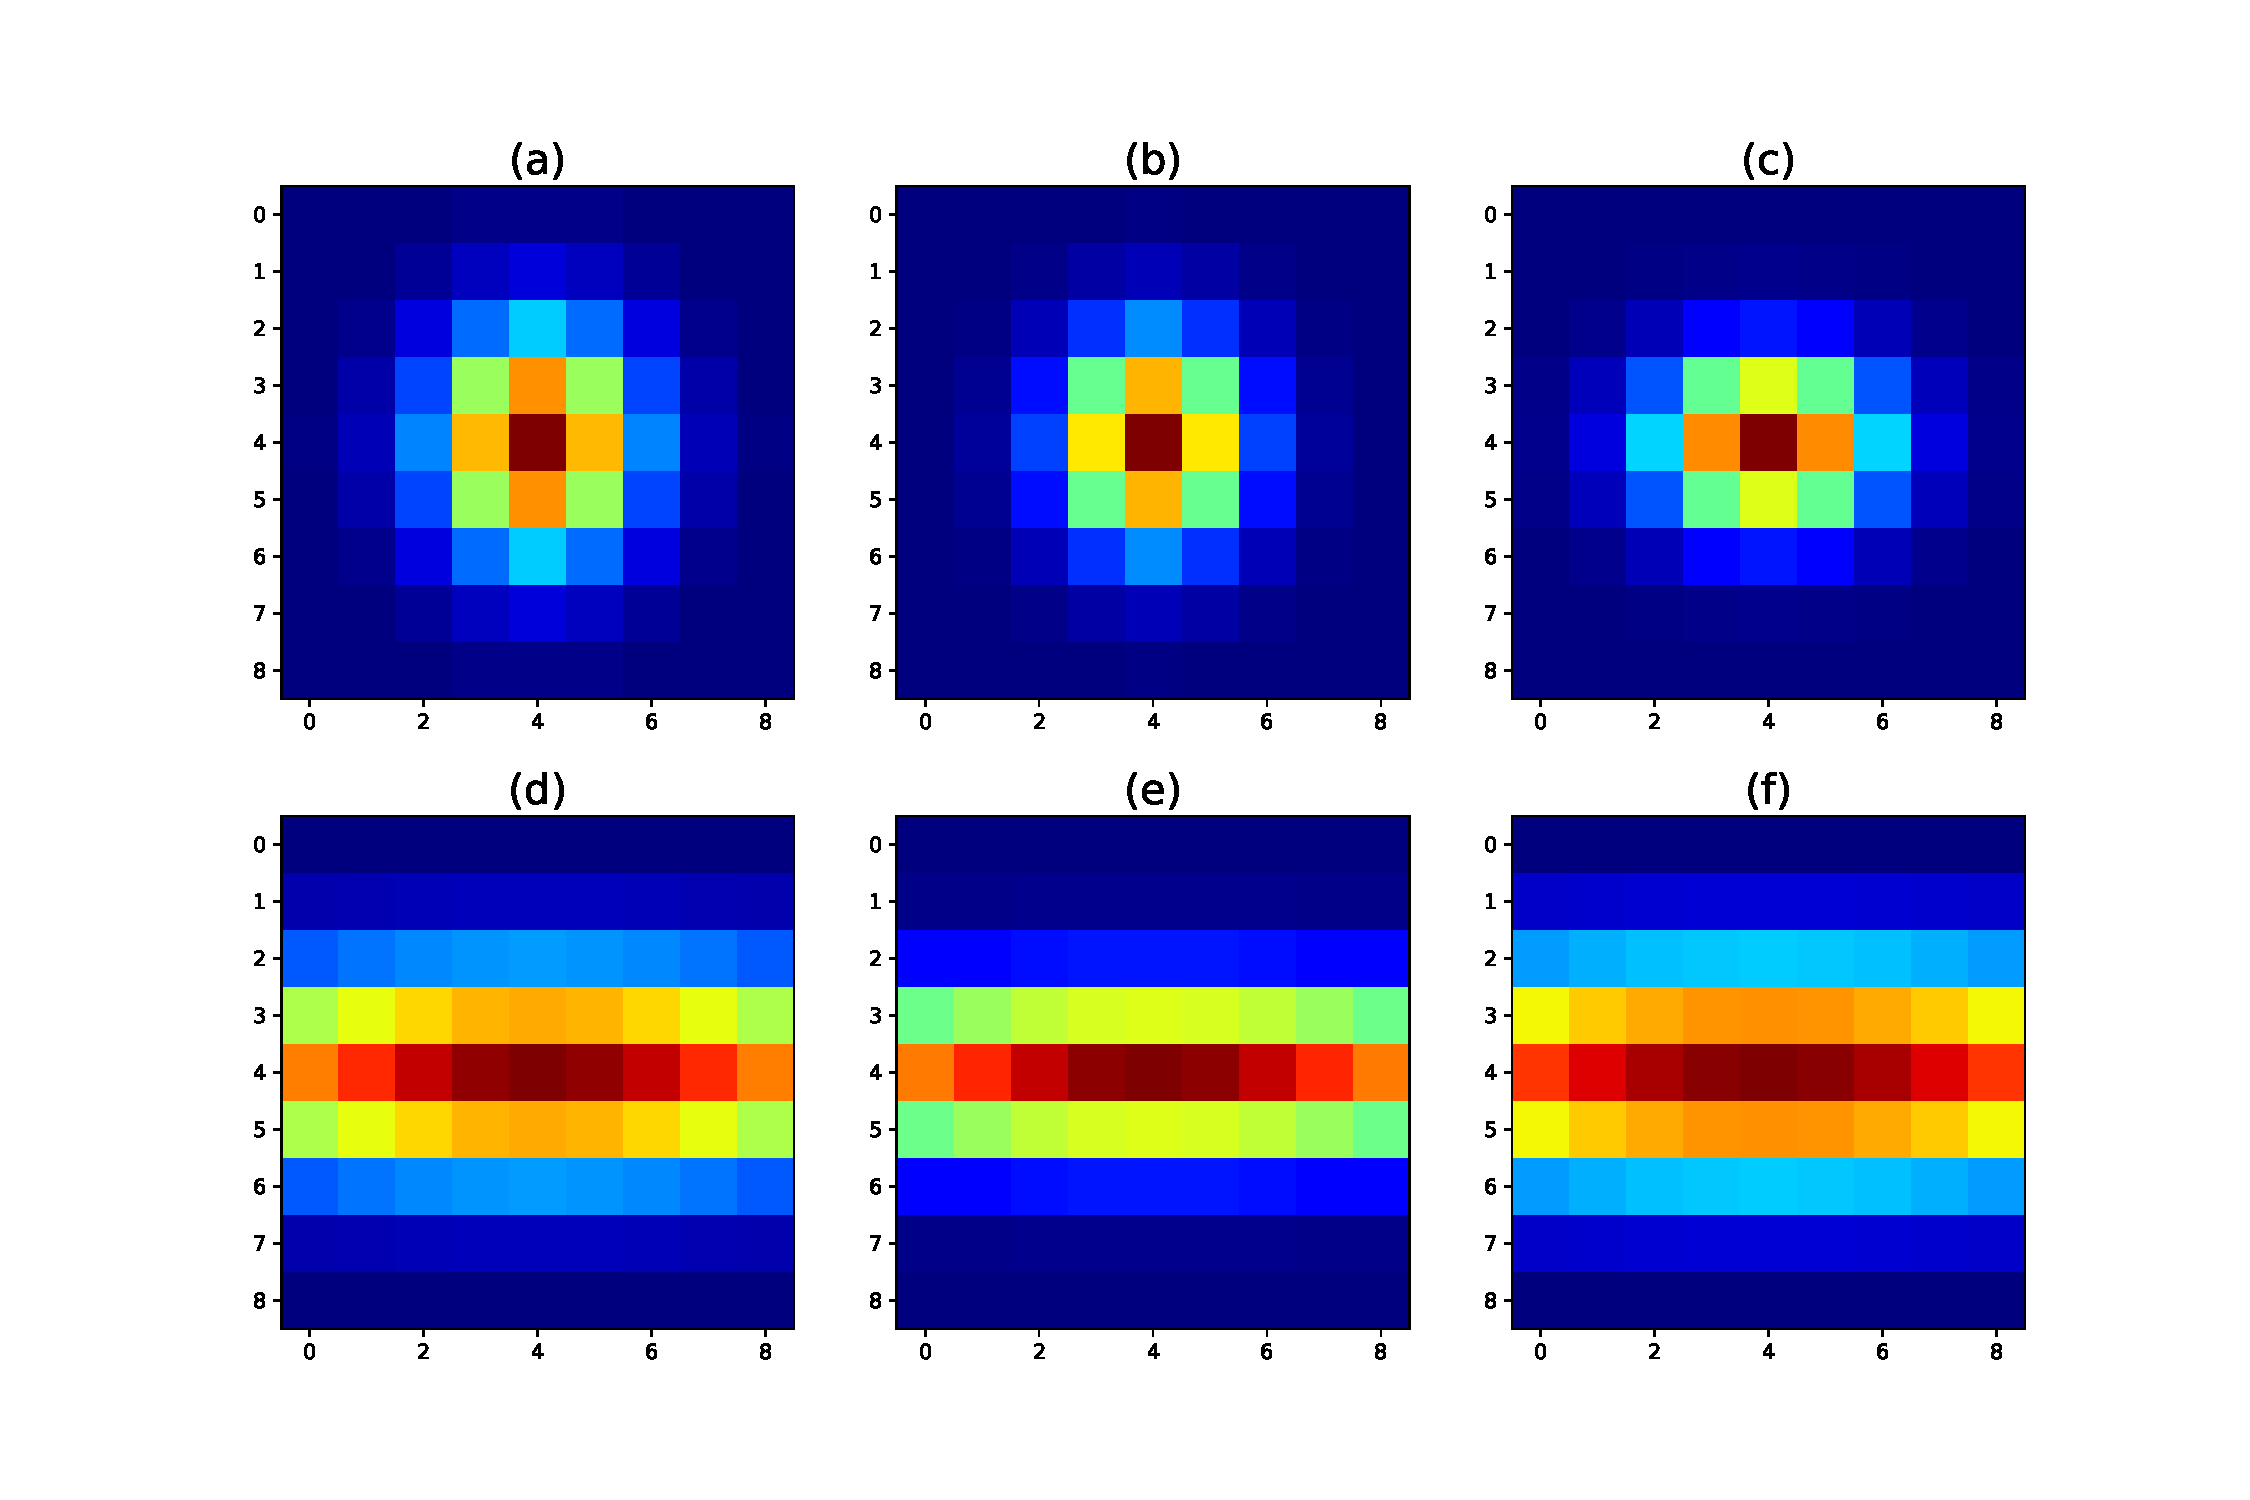
\includegraphics[width=\linewidth]{Includes/4-degradation_kernels.pdf}
                \caption{Example of kernels used in a stochastic degradation model. (a),(b) and (c) are generated using a symmetric variance on the x and y-axis. (d) (e) and (f) are generated using an asymmetric variance, resulting in anisotropic kernels.}
                \label{fig:4-degradation_kernels}
            \end{figure}

        \begin{figure}[H]
                \centering
                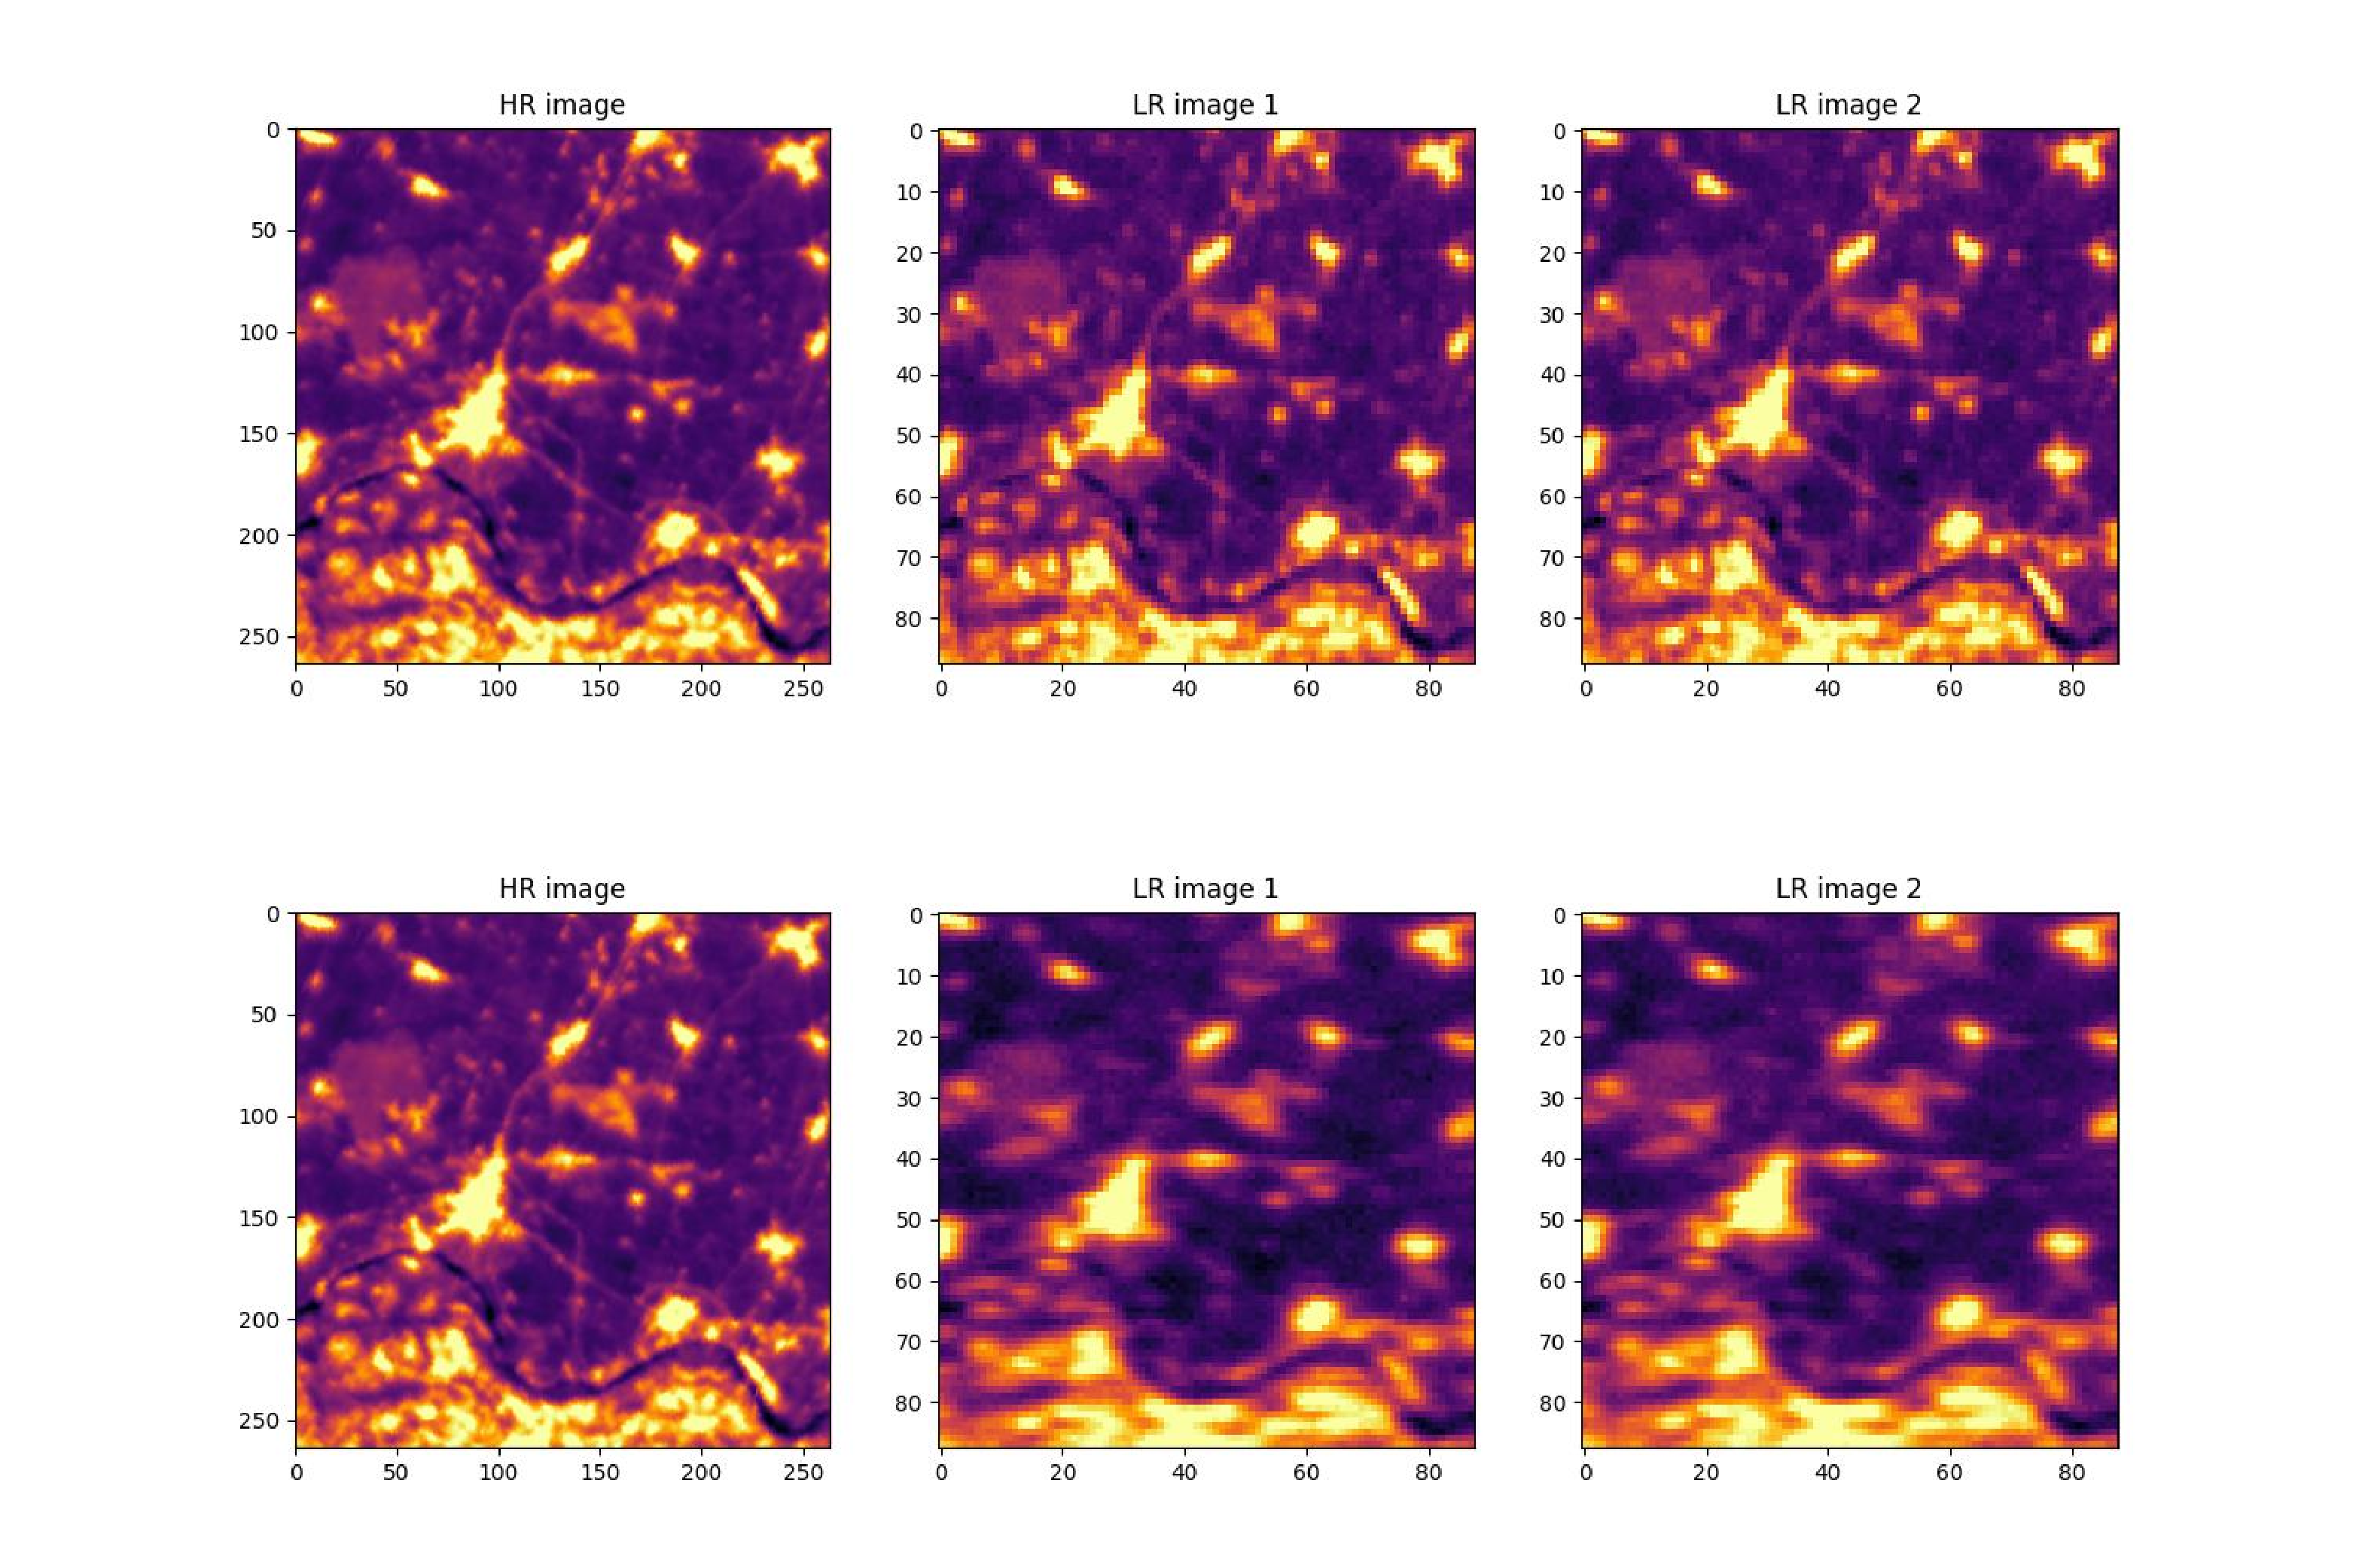
\includegraphics[width=\linewidth]{Includes/4-degradation-kernel-examples.pdf}
                \caption{Effects of different blurring kernels on the HR-LR generation. The upper row contains images generated using blurring kernels with symmetric distributions. The lower rows contain images generated using asymmetric distributions, resulting in highly anisotropic kernels.}
                \label{fig:4-degradation-kernel-examples}
            \end{figure}
            
        \subsubsection{Radiometric error correction}

        FOREST-2 radiometric accuracy is 1K at 300K.
        Other missions report higher nominal radiometric accuracy, such as the case of the ECOSTRESS instrument sheet \cite{ECOSTRESS2023INSTRUMENT}, which is 0.5K at 300K.
        This difference in accuracy should be taken into account. For this, the additional error required is calculated using the following equation:

        \begin{equation}
            e_{\text{forest}} = \sqrt{e_{\text{eco}}^2 + e_{\text{extra}}^2} 
            \label{eq:4-radiometric-error-correction}
        \end{equation}
        
        Where $e_{\text{eco}}$ is the ECOSTRESS error, and $ e_{\text{extra}}$ is the additional error required for FOREST-2.
        
        Using the above equation, an additional radiometric error of approximately 0.8660K is needed. The next step involves converting the extra error into a radiance value, by calculating the derivative of the Planck equation at 300K, which is done numerically as follows:
        
        \begin{equation}
            \frac{\partial B}{\partial T} = \frac{B(\lambda, T + \delta T) - B(\lambda, T)}{\delta T}
            \label{eq:4-planck-derivative}
        \end{equation}  
        
        Multiplying the results of equations \ref{eq:4-radiometric-error-correction} and \ref{eq:4-planck-derivative}, the radiance error for both FOREST LWIR bands is obtained. The additional radiance errors for LWIR1 and LWIR2 bands are found to be \(1.5472 \times 10^{-1}\) W/sr/m\(^2\)/\(\mu m\) and \(1.1444 \times 10^{-1}\) W/sr/m\(^2\)/\(\mu m\), respectively.

        The difference in radiance will be split into two components. On one side, the cold bias represents a systematic error in the measurement; this error acknowledges discrepancies that can be attributed to sensor calibration and atmospheric conditions. On the other side, the random noise accounts for unpredictable fluctuations in the measurement process. This could be due to a variety of sources like electronic noise in the sensor, random atmospheric disturbances, or other stochastic factors. As the extent of each component is not known and to give more variability to this basic degradation model, a random factor $\phi \in [0,1] $ is introduced:

        \begin{equation}
        \begin{aligned}
            \varepsilon_{\text{final}} &= (1 - \phi) \times \varepsilon_{\text{radiance}} + \phi \times \eta \times \varepsilon_{\text{radiance}} \\
            \eta & \sim \mathcal{N} (0,1)
        \end{aligned}
        \end{equation}    

        The effects of the error correction are shown in Fig. \ref{fig:4-radiometric_noise_example}. As the target radiometric error increases, the loss of information is more noticeable.


        \begin{figure}[h!]
            \centering
            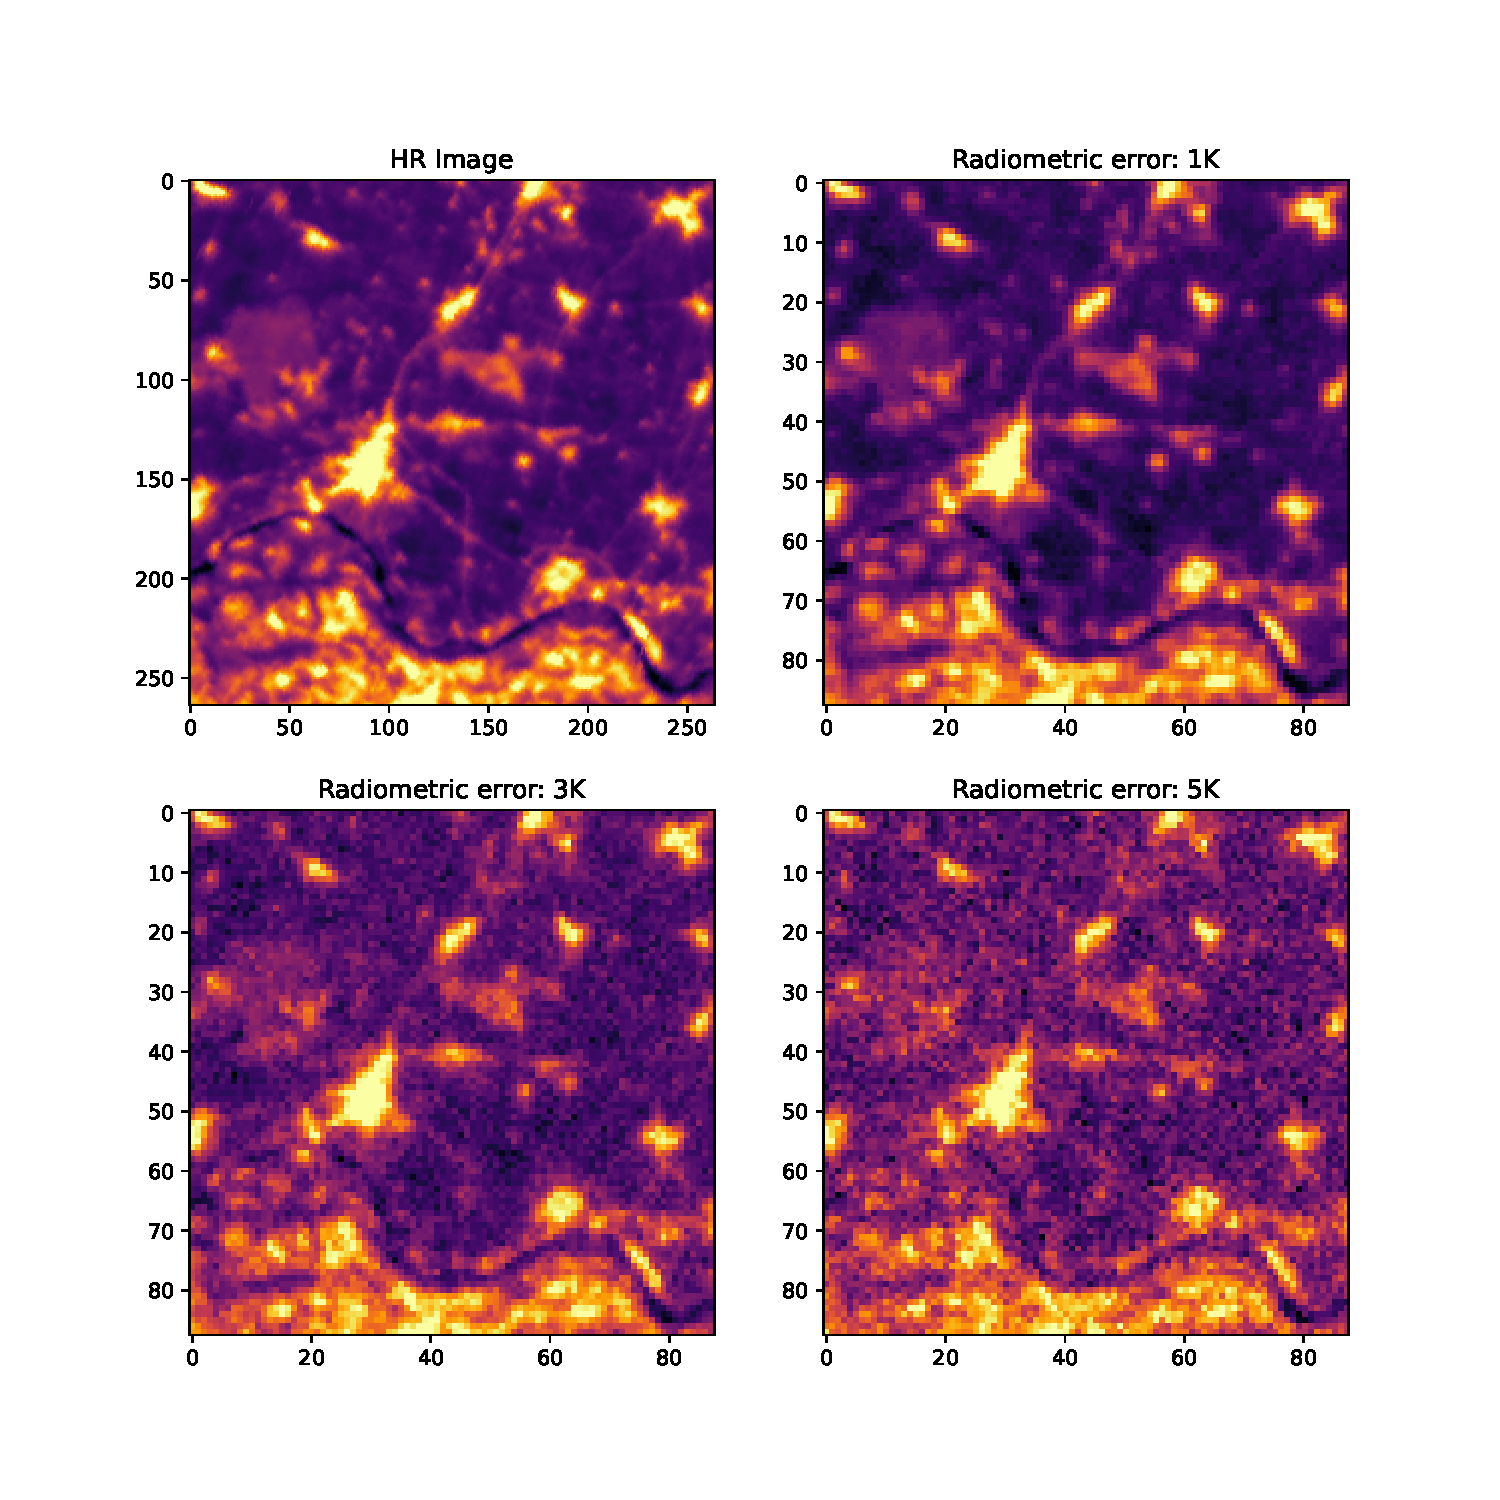
\includegraphics[width=\textwidth]{Includes/4-radiometric_noise_example.pdf}
            \caption{Effects of increasing radiometric error on the HR-LR generation.}
            \label{fig:4-radiometric_noise_example}
        \end{figure}
        
    

    \subsection{Signal-to-noise ratio }

        The Signal-to-Noise Ratio (SNR) is commonly used to quantify how much a signal is corrupted by noise. It is defined as the ratio of signal power to noise power and is usually expressed in decibels (dB). Mathematically, the SNR is often defined as:

        \[ \text{SNR} = 10 \log_{10} \left( \frac{P_{signal}}{P_{noise}} \right) \]

        Where $P_{signal}$ and $P_{noise}$ represent the power of the signal and the noise tensors, calculated as the sum of their squared elements.
        A higher SNR indicates a more distinguishable signal in comparison to the noise. In the context of this work, it will be used to assess the power of the noise introduced by the probabilistic degradation model compared to the clean image.

    \subsection{Referenced image quality metrics}

        When the HR image is available, the performance of a super-resolution algorithm can be evaluated using a variety of metrics. 
        These metrics can be divided into two categories: pixel-based and perceptual-based.
        Pixel-based metrics are based on the pixel-wise comparison between the generated image and the ground truth. 
        Perceptual-based metrics, on the other hand, are based on the perceptual similarity between the generated image and the ground truth. 
        These metrics are built using a pre-trained deep neural network, which is usually trained on a large dataset of images.
        The following sections will describe the most commonly used metrics in the literature.

        \subsubsection{Pixel-wise losses}

            The $L_1$ and $L_2$ losses are the most commonly used pixel-based metrics in the literature. 
            Additionally, they are the most common loss function that drives the super resolution network gradients during training. 
            In a general form, the $L_1$ and $L_2$ losses are defined as follows:

            \begin{equation}
                \mathcal{L}_{L_p} = \frac{1}{H \cdot W} \sum_{i=1}^{H} \sum_{k=1}^{W} |I^{\text{HR}}_{i,k} - I^{SR}_{i,k}|^p
            \end{equation}

            Where $I^{\text{HR}}_{i,k}$ and $I^{SR}_{i,k}$ are the ground truth and the super-resolved image at the pixel position [i,k], and $p$ is the exponent of the loss function. 
            The $L_2$ loss weights high-value differences higher than low-value differences due to the exponent of two, resulting in an excessively smooth loss for low values and considerable variability for high values.
            For that reason, it is more common to see the $L_1$ loss being used in the SR literature and is the one employed in the experiment.

        \subsubsection{Adversarial loss}

        In order to train the probabilistic degradation model GAN, an adversarial loss must be used. 
        Viewing the discriminator as a classifier, the original GAN implementation uses the cross-entropy loss. This will cause the problem of vanishing gradients in the generator when the samples are on the correct side of the decision boundary but are still far from the real data. For that reason, the LSGAN is proposed in \cite{mao2017squares}. 
        
        Benefits of LSGANs include the penalization of samples that are on the correct side of the decision boundary but far from it. This will generate more considerable gradients in the generator update, relieving the vanishing gradients problem. As a result, the learning process is more stable and will create higher quality images from the generator.

        

        \subsubsection{Peak signal-to-noise ratio}

         
            Peak Signal-to-Noise Ratio (PSNR) measures the magnitude of the error compared with the reference image. It is usually used to quantify the amount of error or noise introduced during the image reconstruction process.
            
            PSNR is calculated by first computing the Mean Squared Error (MSE) or $\mathcal{L}_2$ loss between an image and the reference and then taking the logarithmic ratio of the maximum possible pixel value squared. The PSNR value is usually expressed in decibels (dB). The formula for PSNR is:
            
            \begin{equation}
            PSNR = 10 \cdot \log_{10} \left( \frac{I_{MAX}^{2}}{\mathcal{L}_2} \right)
            \end{equation}
            
            Where $I_{MAX}$ is the maximum possible pixel value of the reference image, and $\mathcal{L}_2$ is the mean squared error between the image and the reference. A higher PSNR value indicates a better quality of the super-resolved image, as it signifies a lower level of noise or error. However, it's worth noting that it may not always align with human perceptual evaluations of image quality, as it focuses on physical consistency.

        \subsubsection{Structural similarity index}

            
        Structural Similarity Index Measure (SSIM) takes into consideration changes in structural information, luminance, and contrast. By doing this, it manages to reflect the perceived changes in noise level and contrast better.
        The SSIM index is calculated by dividing the image into windows of a certain size and then comparing corresponding windows in the reference and target images. The SSIM index for a pair of windows, say $x$ and $y$, is given by:
        
        \begin{equation}
            SSIM(x, y) = \frac{(2\mu_x\mu_y + c_1)(2\sigma_{xy} + c_2)}{(\mu_x^2 + \mu_y^2 + c_1)(\sigma_x^2 + \sigma_y^2 + c_2)}
        \end{equation}
        
        Where $\mu_x$ and $\mu_y$ are the average pixel values, $\sigma_x^2$ and $\sigma_y^2$ are the variances, $\sigma_{xy}$ is the covariance of $x$ and $y$, and $c_1, c_2$ are small constants to avoid division by zero.
        The final SSIM score for the images is calculated by averaging the SSIM indices of all windows. An SSIM score of 1 indicates a perfect structural match between the two images, whereas a score of 0 indicates no structural similarities.

        \subsubsection{Learned perceptual image patch similarity}

        LPIPS is a perceptual metric that leverages deep learning to compute perceptual differences between images. Specifically, it uses the activations of a pre-trained convolutional neural network (in this case, VGG \cite{VGGnet} ) to extract perceptual features from the images afterwards. 
        Then, it calculates the Euclidean distance between these feature vectors to measure the perceptual difference.
        This measure has gained popularity in SR tasks due to its high correlation with human judgments of visual similarity \cite{zhang2018unreasonable}.
        
        The LPIPS score is given by:
        
        \begin{equation}
        LPIPS(I^{HR}, I^{SR}) = \sqrt{\sum_{i=1}^{N} w_i\|f_i(I^{HR})-f_i(I^{SR})\|^2}
        \end{equation}
        
        where $I^{HR}$ and $I^{SR}$ are the images being compared, $f_i(I)$ denotes the $i$-th layer activation when image $I$ is the input to the pre-trained network, $N$ is the number of layers considered, and $w_i$ is the learned weight for the $i$-th layer.
        
        A lower LPIPS score indicates a lower distance between the feature vectors and, thus, a greater perceptual similarity between the two images. 
        Due to the fact that in this work, we are interested in the physical consistency of the super-resolved images, 
        this metric will be shown but will not drive any decision during the training process.
        

        \subsubsection{Translation and bias adjustment}\label{subsec:adjustedmetrics}
    
            In order to calculate the losses and performance metrics, the generated test images are compared against the HR images.
            Additional changes should be considered, particularly in a MISR environment \cite{martens2019superresolution}.
            Minor shifts in the contents of the pixels are expected, and  SR methods may have undesired effects on the border pixels. Therefore, metrics should have some tolerance to small pixel translations in the high-resolution space by evaluating a sliding cropped image. 
            This implies looking for a displacement of SR by at most $d$ pixels in each direction and picking the one that minimizes the error. 
            An example of how this is applied in a loss that needs to be minimized can be found in Eq. \ref{eq:4_adjusted_metrics}
    
            \begin{equation}
               \mathcal{L}^* ( I^{HR}, I^{LR}, d) = \min_{u,v \in [0,2d]} \mathcal{L} ( I^{HR}_{u,v}, I^{SR}_{u,v})
            \label{eq:4_adjusted_metrics}
            \end{equation}
    
            Additionally, commonly used metrics punish biases as much as noise in the reconstruction.
            For example, if $I^{SR} = I^{HR} + \epsilon$, where $\epsilon$ is a constant bias, a perfect reconstruction of $I^{SR}$ is possible if $\epsilon$ is known. 
            A quality metric should award a high score to super-resolved outputs with these characteristics in comparison to the introduction of noise and information loss. Metrics like L2/L1 losses and PSNR do the exact opposite and thus should incorporate a bias compensation like the following: 
    
            \begin{equation}
                \begin{aligned}
                    \mathcal{L}^* ( I^{HR}, I^{LR}, d) = \min_{u,v \in [0,2d]} \mathcal{L} ( I^{HR}_{u,v}, (I^{SR}_{u,v}+b)) \\
                    b = \frac{1}{(W - d)(H - d)} \sum_{x,y} \left( I^{HR}_{u,v} - I^{SR}_{u,v} \right)
               \end{aligned}
            \end{equation}
    
            \noindent Where $W$ and $H$ represent the width and height of the image, respectively.
    

    \subsection{Non-referenced image quality metrics}

    Non-Referenced Image Quality Assessment (NRIQA) aims to develop methods to measure image quality in alignment with human perception without the need for an HR reference. 
    Most of them are based on two steps: feature extraction and quality prediction using a regression module. 
    They rely on the assumption that natural images share certain statistical information and that any distortion may alter these statistics \cite{niqe}.
    The results from an arbitrary image are compared to a default model trained on a large dataset of natural scenes, and the difference between them is used to predict the quality of the image.
    % In recent years, researchers have relied on deep learning to perform the two steps in a single model. 
    % The workflow of these models is shown in Fig. \ref{fig:4-nr-iqa-workflow}.

    % \begin{figure}[h!]
    %     \centering
    %     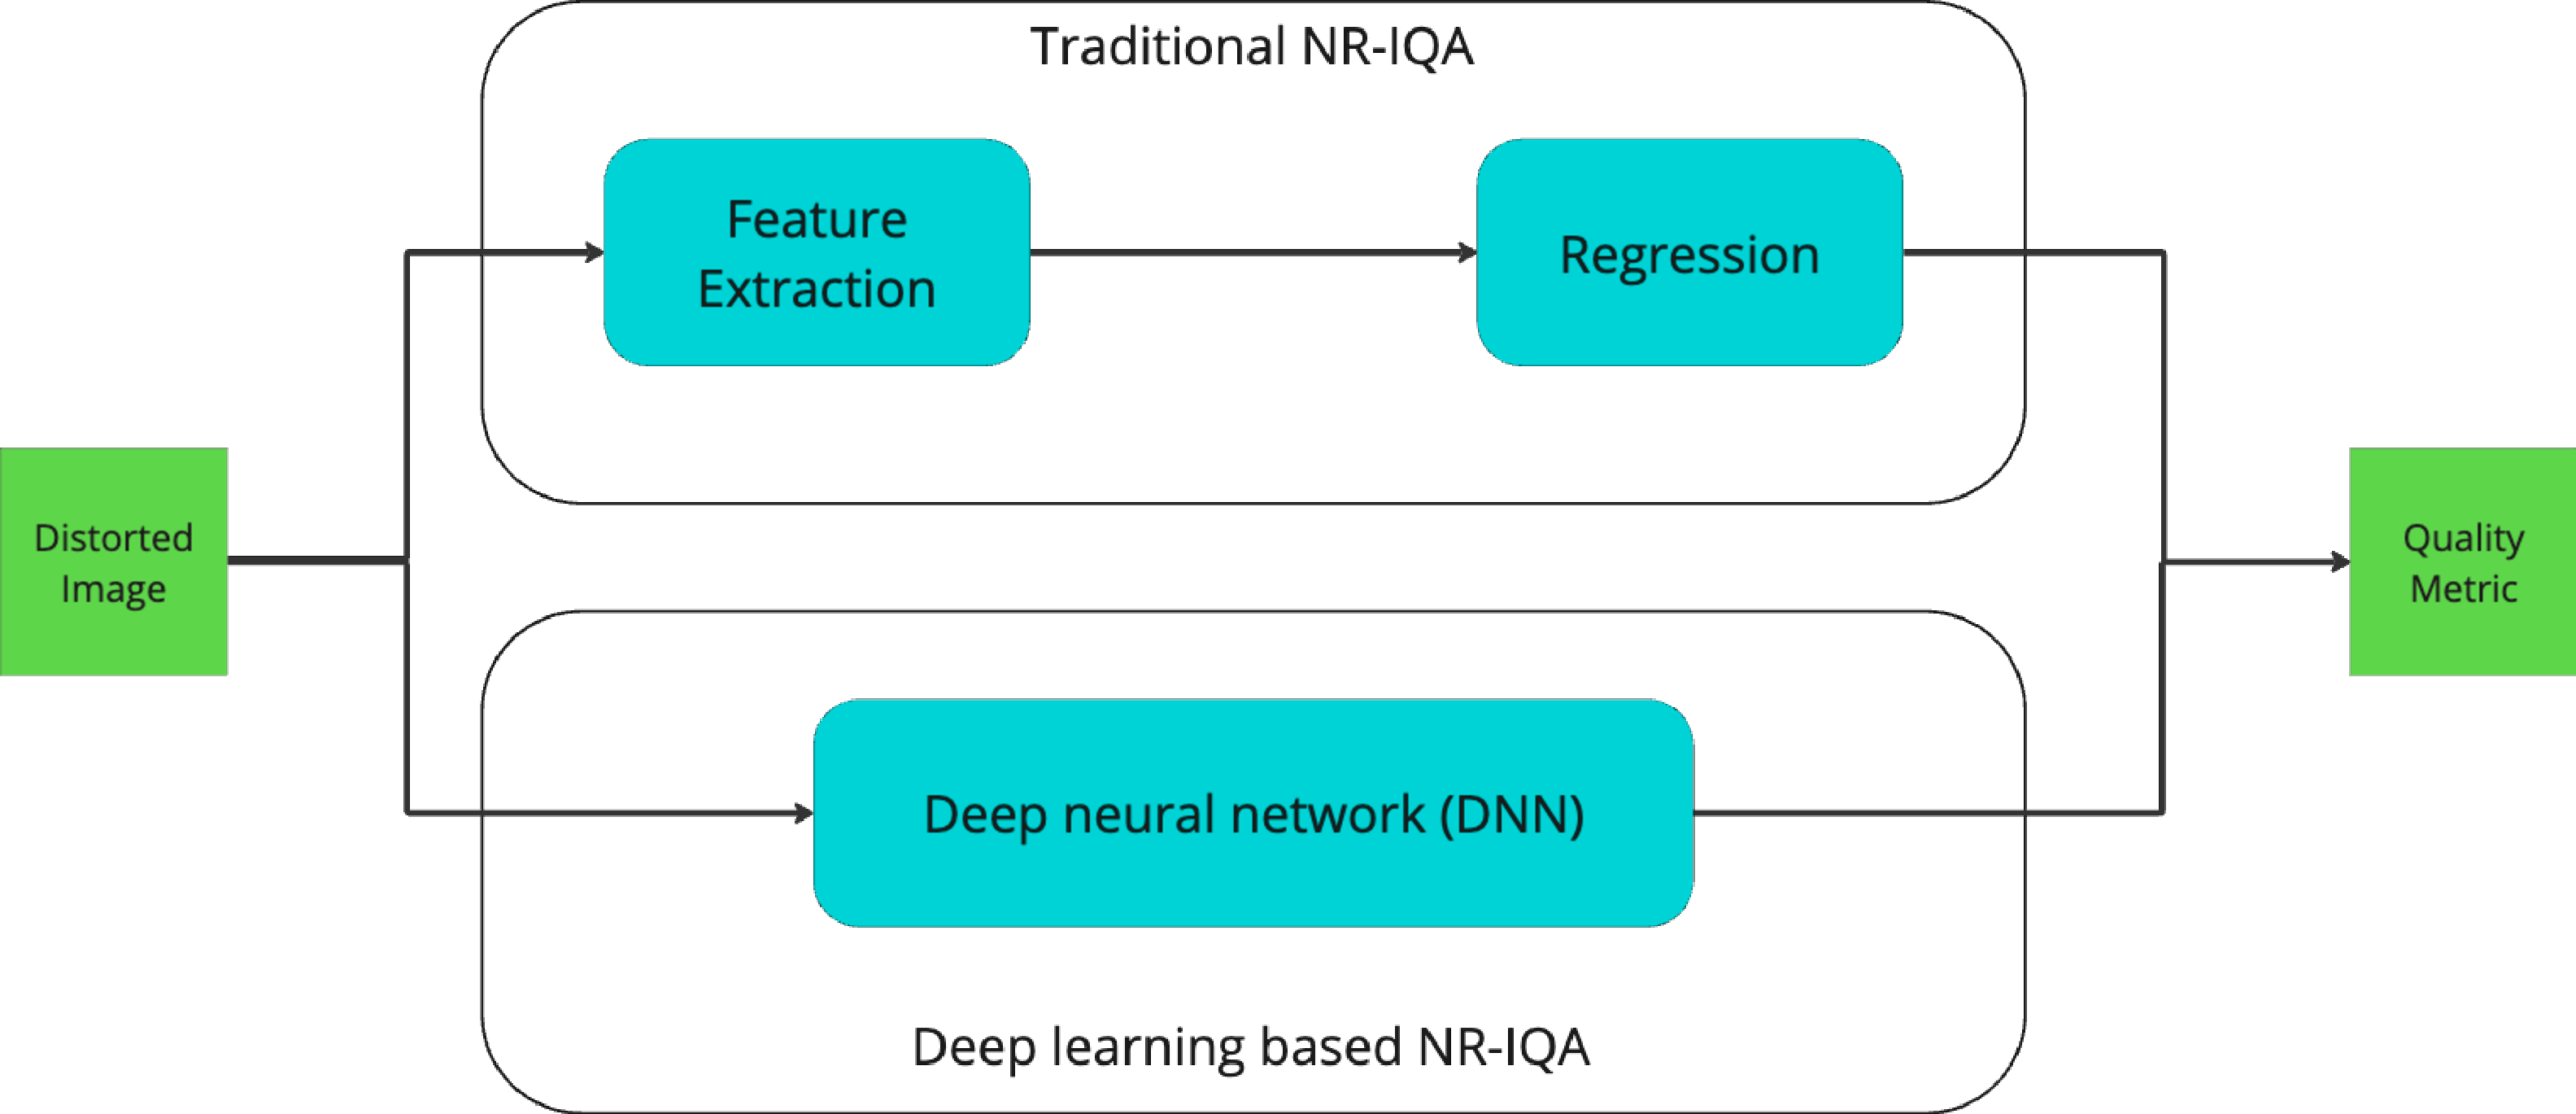
\includegraphics[scale=0.25]{Includes/3-NR-IQA.pdf}
    %     \caption{Workflow of an NR-IQA model.}
    %     \label{fig:4-nr-iqa-workflow}
    % \end{figure}


        

        \subsubsection{Naturalness image quality evaluator}

        
            The Naturalness Image Quality Evaluator (NIQE) \cite{niqe} operates on the principle that pristine natural images exhibit specific statistical properties that can be quantified to establish a benchmark for quality assessment. 
            NIQE employs a model based on a multivariate Gaussian distribution characterized by a mean vector and covariance matrix to represent the statistical attributes of a natural image's visual patterns.
            To assess its quality, NIQE extracts a corresponding set of features and evaluates their deviation from this statistical model using the Mahalanobis distance.
            This distance measures the divergence of the image's features from those typical of high-quality natural images.
            A lower value suggests that the image closely resembles the statistical properties of natural images, indicating higher perceived quality. This provides a measure of image quality that aligns with the naturalness of human visual perception. 

        \subsubsection{Blind/referenceless image spatial quality evaluator}

            Similar to NIQE, the Blind/Referenceless Image Spatial Quality Evaluator (BRISQUE) \cite{mittal2012} operates on the premise that natural images possess specific statistical properties that are altered in the presence of distortions. It operates by quantifying deviations from the statistical regularities observed in natural images, primarily using locally normalized luminance coefficients. 
            Following this, a spatial domain model is utilized to calculate a set of features that are designed to capture the loss of naturalness due to the presence of distortions.
            These extracted features are fed into a Support Vector Regression (SVR) that was trained with a set of images with known quality ratings to predict the quality score of the image.
            
            A lower BRISQUE score is indicative of better quality, implying that the image has a better quality score in the pre-trained model. The main difference between BRISQUE and NIQE is that BRISQUE uses the SVR model and directly predicts the quality score, while NIQE calculates the distance between the multivariate Gaussian distribution model of the image and the one from the specific dataset where the evaluator was pre-trained.




        \subsection{Frequency domain analysis} \label{subsubsec:frequency_domain_analysis}
        
        The Fourier transform is widely used to analyze the frequency content of signals.
        It can also be applied to multidimensional signals such as images, where the spatial variations of pixel intensities have a unique representation in the frequency domain. 
        The objective of the super resolution is to reconstruct missing high-frequency components from an LR image.
        A good SR algorithm seeks to amplify the high-frequency components compared to a baseline such as bicubic interpolation while keeping noise at bay.
        The Fourier components provide global information about the image, as opposed to local information represented by pixel values in the spatial domain \cite{fuoli2021fourier}. 
        
        Using the Fast Fourier Transform (FFT), the pixel intensity values of super-resolved images are converted into a spectrum where each point represents a specific frequency contained in the spatial domain.
        The FFT is then shifted so that the zero-frequency component is at the center of the spectrum. 
        The resulting magnitude reveals the energy distribution across various frequencies and is usually visualized in grayscale, where the intensity corresponds to the amplitude of the frequency components.
        
        A radial profile of the FFT magnitude provides insights into how different spatial frequencies contribute to the image content.
        The radial profile calculates the average intensity of frequencies at a given radius from the center of the Fourier transform and depicts the average magnitude of a given frequency in all possible directions. This metric serves as a benchmark for evaluating the performance of SR techniques against traditional interpolation methods such as bicubic interpolation.
        
        Spatial frequency within an image context refers to the periodicity of the intensity variation over spatial dimensions, typically quantified in cycles per pixel. The central region of the frequency domain, after the shift operation, denotes the zero frequency. In contrast, the edges of the FFT image represent the highest frequencies, constrained by the image's discrete sampling rate.
        To quantitatively interpret these spatial frequencies, a radial-to-frequency mapping is necessary. This mapping accounts for the Nyquist frequency, which is delineated as half the sampling rate of the discrete imaging grid composed of squared pixels.

        It is important to note that given the 2D nature of an image, the Nyquist limit is not the same in all directions. 
        Along each axis, the Nyquist limit is 0.5 cycles per pixel. Still, in a diagonal direction, the limit is reached by combining the spatial frequency of the $x$ and $y$ axis, which is at $\frac{\sqrt{2}}{2} \approx 0.707$ cycles per pixel. 
        This means that frequencies above 0.5 cycles per pixel can be detected only if their direction is not along any of the axes.
        The effect of the Nyquist limit can be seen in Fig. \ref{fig:5-square_vs_radial}. The maximum possible frequency in an FFT plot of a squared image is in the corners. However, when normalized by the direction-dependent Nyquist limit, the maximum is reached in the borders of the FFT.

        \begin{figure}[H]
            \centering
            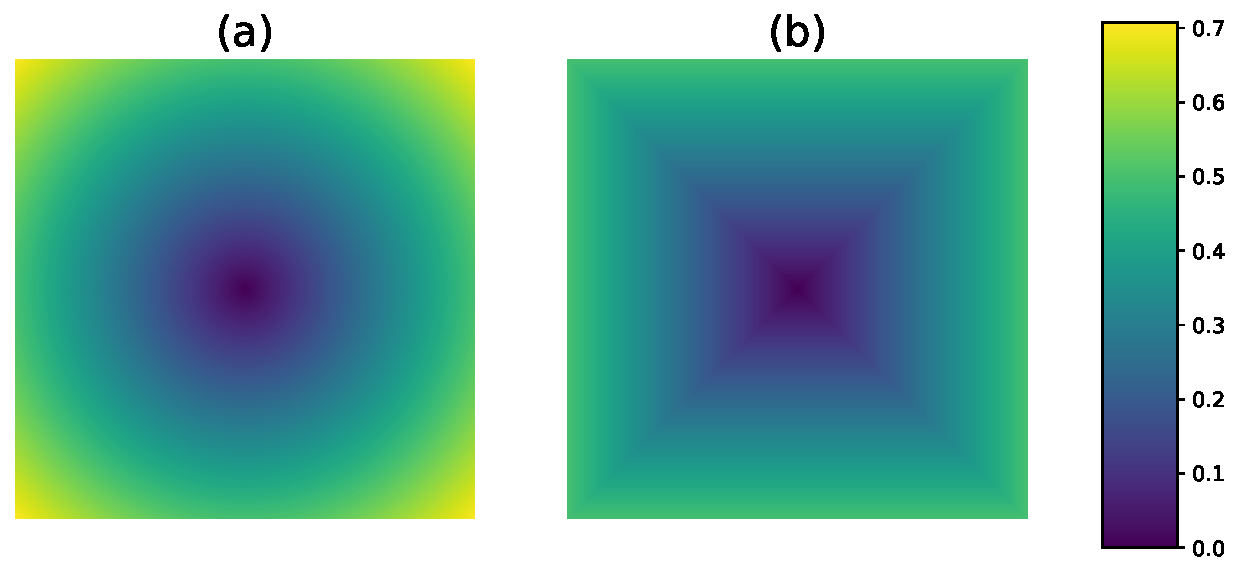
\includegraphics[width=\linewidth]{Includes/5-square_vs_radial.pdf}
            \caption{Comparison between (a) the radial representation of frequencies in cycles per pixel and (b) the frequency normalized by the direction-dependent Nyquist limit. The frequency limit is always on the borders of the FFT plot, but they represent different frequency values depending on the direction.
            }
            \label{fig:5-square_vs_radial}
        \end{figure}
        
        
        The conversion of a given radius in the FFT output to the corresponding spatial frequency is formalized as:

        \begin{equation}
            f(r) = \frac{r}{\frac{N}{2}} \cdot f_{\text{Nyquist}},
        \end{equation}

        Where \( f(r) \) signifies the spatial frequency associated with radius \( r \), \( N \) represents the FFT image dimension, assuming a square configuration, and \( f_{\text{Nyquist}} \) the Nyquist frequency, which is 0.5 cycles per pixel along the $x$ and $y$. An example of the procedure is shown in \ref{fig:4-frequency-analysis}. Usually, frequencies higher than 0.5 cycles per pixel have a low log magnitude and can be disregarded in the analysis.

        \begin{figure}[H]
            \centering
            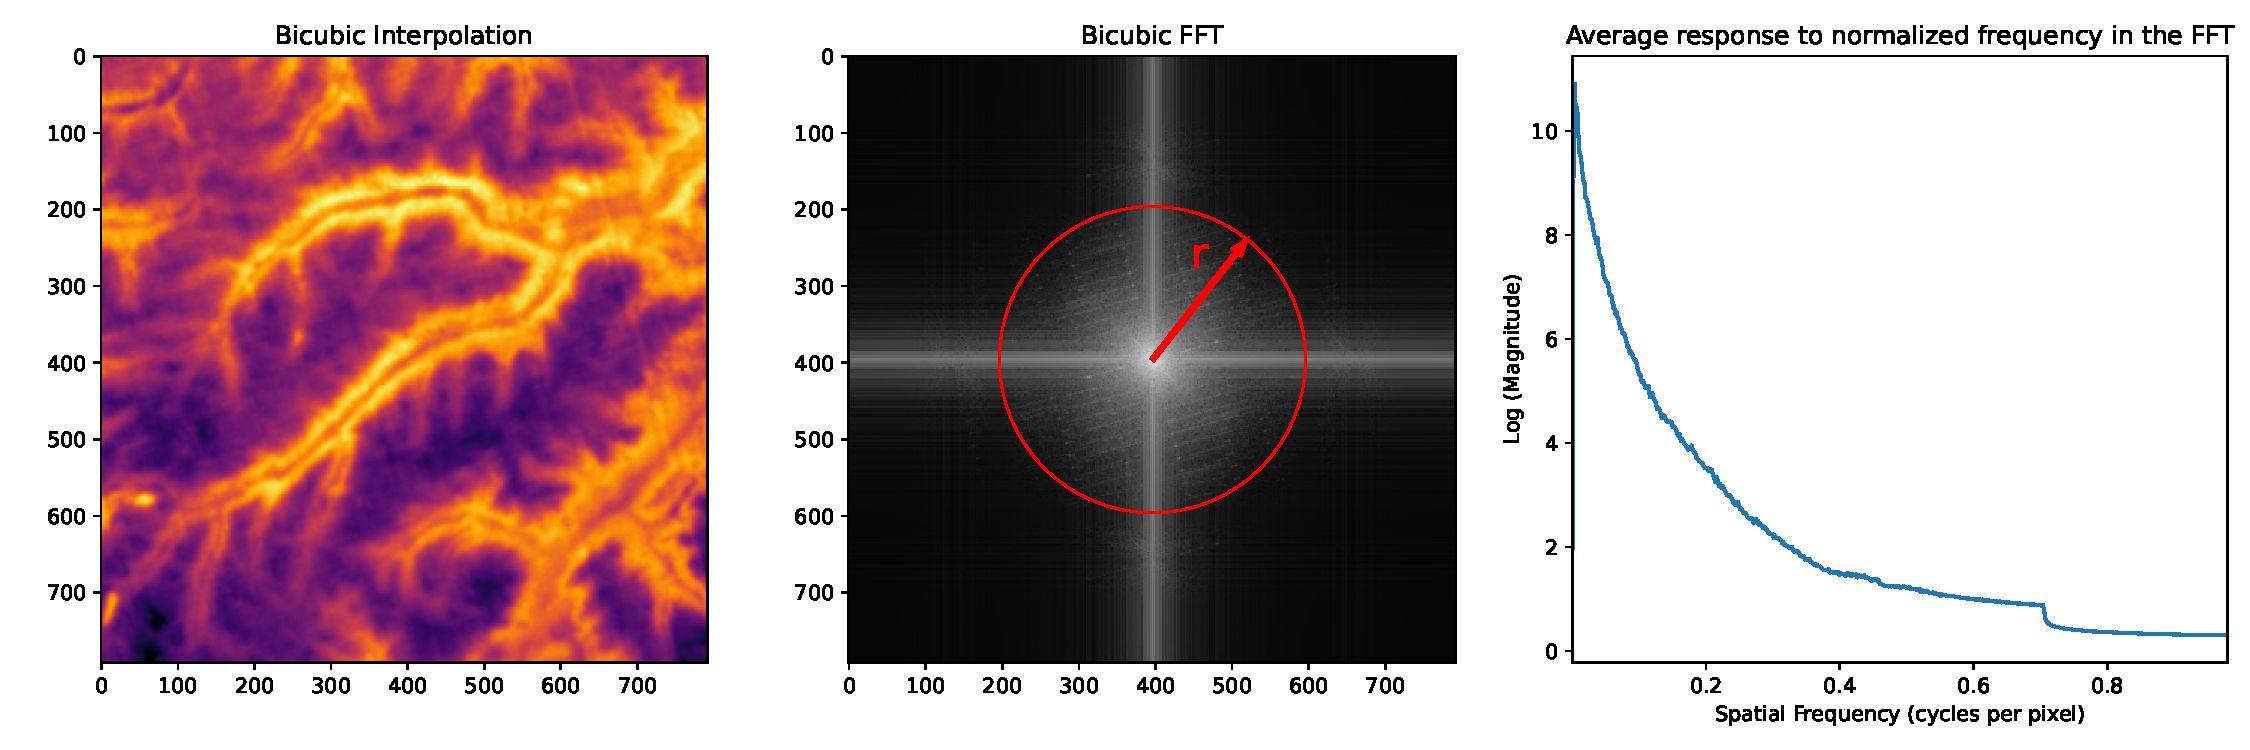
\includegraphics[width=\linewidth]{Includes/4-frequency-analysis.pdf}
            \caption{Steps of the frequency domain analysis. (b) shows the log magnitude of the shifted FFT of the scene depicted in (a). The radial profile is calculated by averaging all the points that have the same $r$. In (c), the log magnitude obtained for every radial profile is plotted, translating the axis from radius into spatial frequency.}
            \label{fig:4-frequency-analysis}
        \end{figure}
        

        Through FFT, a depiction of the amplification or attenuation of frequencies attributable to the SR techniques can be calculated. 
        Analyzing these profiles displays the ability of SR models to enhance details. 
        However, it is essential to note that this method does not account for artifacts generated by the super resolution process and should be used in combination with other metrics.

        \subsection{Gradient distribution analysis}


        An alternative way of analyzing super resolution results is by looking at the gradients of the images. 
        HR images are sharper, and thus, each pixel on average, has higher gradient magnitudes in both directions compared to their LR counterparts.
        A super-resolution algorithm should increase the sharpness of the edges, resulting in a gradient distribution that aligns more closely with that of the genuine HR image.
        
        An approximation of the gradients can be estimated by doing 2D convolutions between an image and Sobel kernels, as displayed in Eq. \ref{eq:4-sobel-operators} \cite{Sobel1990AnI3}.
        These kernels are designed to respond maximally to edges running vertically and horizontally relative to the pixel grid.
        
        \begin{equation}
            \begin{array}{ccc}
            \hat{G}_x = \begin{bmatrix}
            -1 & 0 & +1 \\
            -2 & 0 & +2 \\
            -1 & 0 & +1
            \end{bmatrix}
            &
            \quad
            &
            \hat{G}_y = \begin{bmatrix}
            +1 & +2 & +1 \\
             0 &  0 &  0 \\
            -1 & -2 & -1
            \end{bmatrix}
            \end{array}
            \label{eq:4-sobel-operators}
        \end{equation}
    
         The kernels can be applied separately to the input image to produce the component of the gradient in each orientation $G_x$ and $G_y$. The magnitude of the gradient  is given by: 
         \begin{equation}
             |G| = \sqrt{G_x^2 + G_y^2}
             \label{eq:4-gradient_magnitude}
         \end{equation}

         The gradient magnitude histograms of the results of different super resolution algorithms will be assessed, thereby quantifying the enhancement in edge sharpness.
         This histogram provides insights into the frequency and intensity of the edges within an image.
         A better SR model should demonstrate a histogram with larger gradient magnitudes, indicating sharper edges.
         However, it is important to note that this analysis is unsupervised and disregards the effect of noise and artifacts introduced during the super-resolution process. Thus, it should be considered in combination with other metrics.

         \begin{figure}[H]
             \centering
             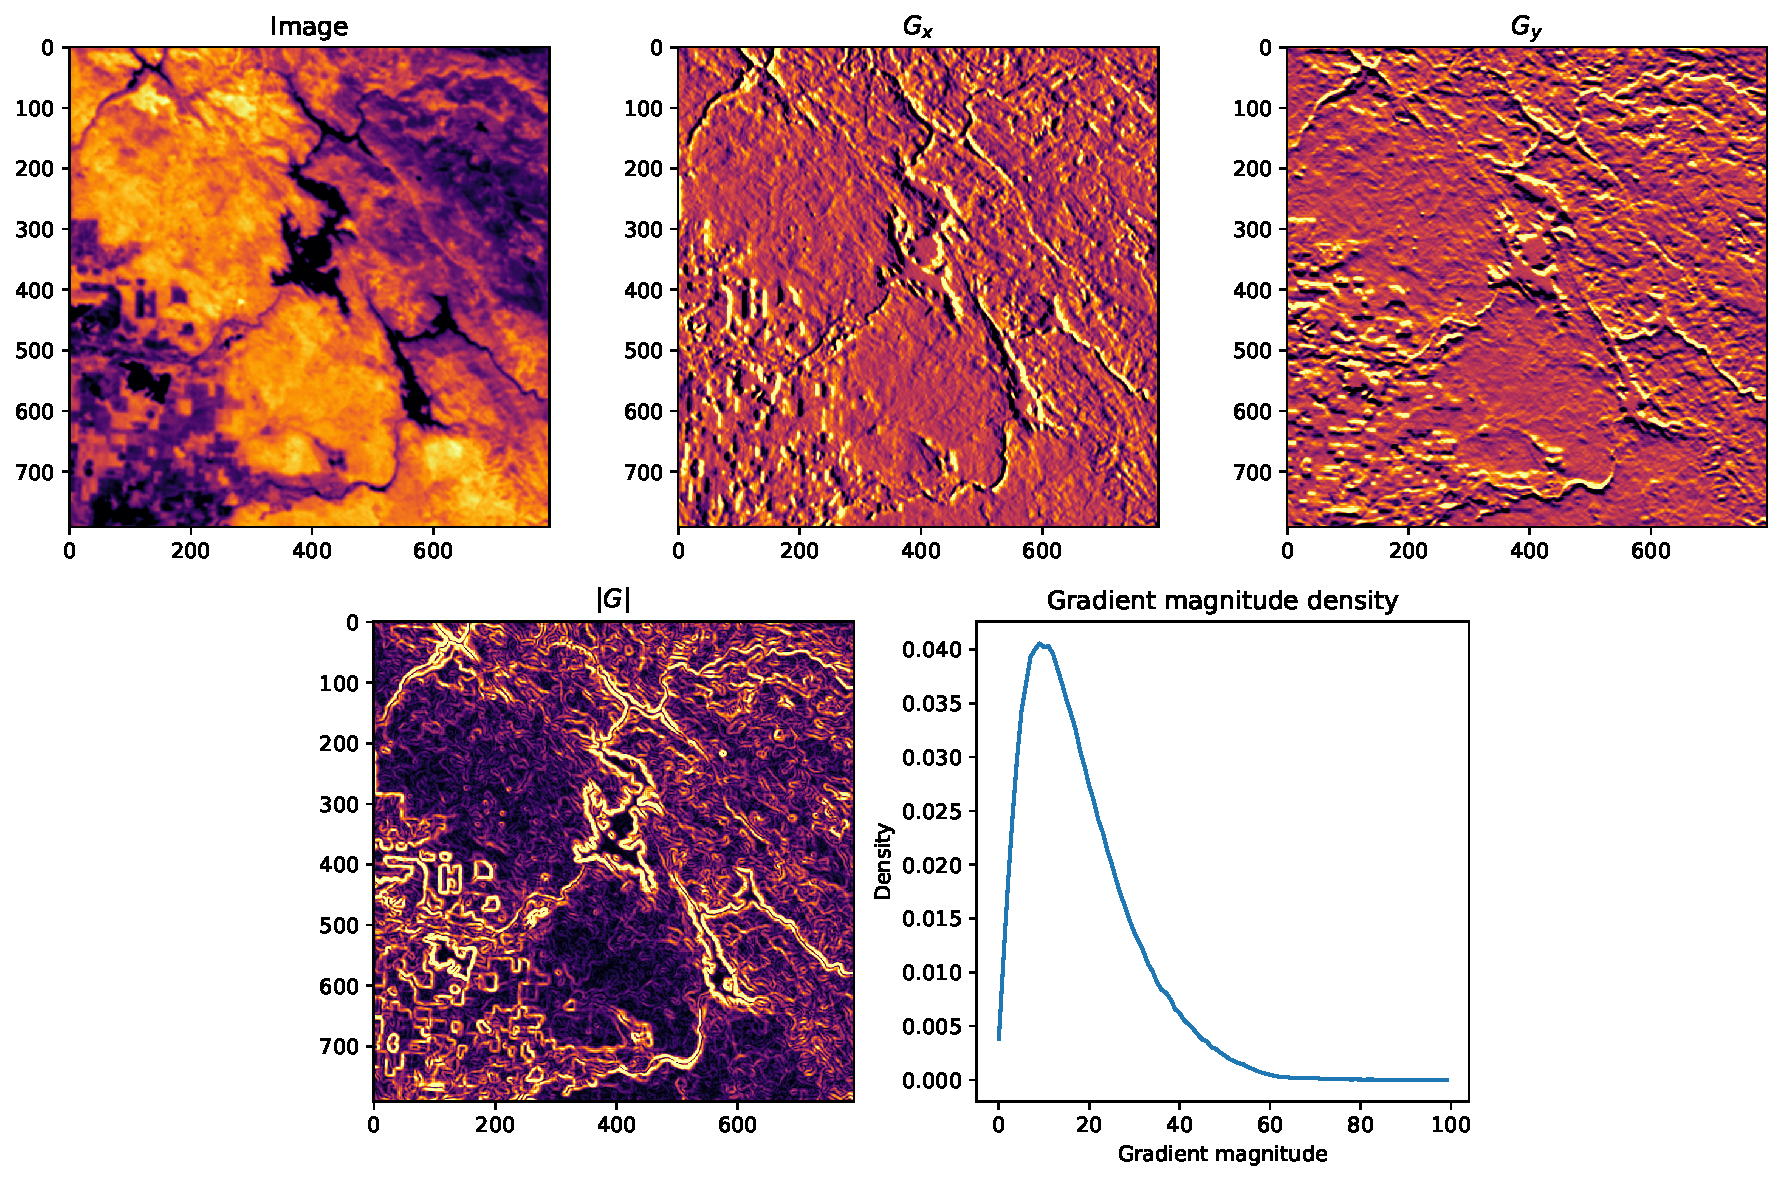
\includegraphics[width=\textwidth]{Includes/4-gradient-analysis.pdf}
             \caption{Steps to obtain a gradient magnitude density. Using the Sobel operators, $G_x$ and $G_y$ are obtained from an image. The magnitude $|G|$ of each pixel is calculated using Eq. \ref{eq:4-gradient_magnitude}. The density can be estimated afterward, using 100 bins in this case.}
             \label{fig:4-gradient-analysis}
         \end{figure}


      \subsection{Correlation between pixel and neighbors }


        In a similar fashion to the gradient analysis, kernels can be used to estimate the correlation between the pixels of an image and their neighbors. The Pearson correlation coefficient between the results of the convolutions of the image and the following kernels will be calculated.
        
        \begin{equation}
            \begin{array}{ccc}
            \hat{G}_{center} = \begin{bmatrix}
            0 & 0 & 0 \\
            0 & 1 & 0 \\
            0 & 0 & 0
            \end{bmatrix}
            &
            \quad
            &
            \hat{G}_{neighbors} = \begin{bmatrix}
             1/8 &  1/8 & 1/8 \\
             1/8 &  0 & 1/8 \\
            1/8 & 1/8 & 1/8
            \end{bmatrix}
            \end{array}
            \label{eq:4-correlation-operators}
        \end{equation}
    
         In an image, a high correlation coefficient is expected, as the content of a pixel is highly dependent on its neighbors. However, images with higher definition have sharper edges, and thus, their correlation coefficient should be lower in comparison. It is important to note that this analysis does not take into account the noise present in the image, as it will reduce the correlation coefficient without improving the image quality. In an extreme case, an image composed only of white noise would have a correlation coefficient between each pixel and its neighbors of 0. Despite this, it is helpful to understand the super resolution process.
         

\clearpage

        

        
        
